\documentclass[11pt,a4paper]{article}
\usepackage[utf8]{inputenc}
\usepackage{amsmath}
\usepackage{amsfonts}
\usepackage{amssymb}
\usepackage{graphicx}
\usepackage{tikz}
\usepackage[left=2cm,right=2cm,top=2cm,bottom=2cm]{geometry}
\author{Paul LANDRIER}
\title{Généralisation des réseau de neurones par l'algèbre différentielle}
\date{}

\usetikzlibrary{shapes}


\newcommand{\R}{\ensuremath{\mathbb{R}}}
\newcommand{\mathcla}{\cal}

\newtheorem{definition}{Definition}

\begin{document}

\maketitle

\section{Introduction}

On cherche à abstraire le fonctionnement d'un réseau de neurones. On se fonde sur l'approche des graphes de calcul.

\section{Solution simpliste}

	La solution la plus simple, n'utilisant pas l'algèbre différentielle, consiste à séparer les annotations en deux types, un pour les fonctions et un pour les dérivées partielles.
	
	Formellement, on définit un monoïde de fonction $(F,\circ,id)$ et semi-anneau $(S,+,\cdot,0,1)$ représentant les dérivées partielles. On annote alors les arrêtes $(u,v)$ du graphe avec $F \times S$, où le premier élément du couple représente la fonction permettant de passer de $u$ à $v$ et le second représente la valeur de la dérivée de cette fonction (on considère exclusivement des fonctions $\R \to \R$, lorsque l'on a besoin de fonctions de plusieurs variable, comme $+$, on précise l'annotation sur le n\oe ud correspondant).\\

	Prenons l'exemple du calcul de la fonction $f(x)=e^{x^2}(x^2 + 2(x + 1))$, représenté par le graphe :\\
	
	\begin{figure}[!h]
	\label{fig:graphe_calc_ex}
	\centering
	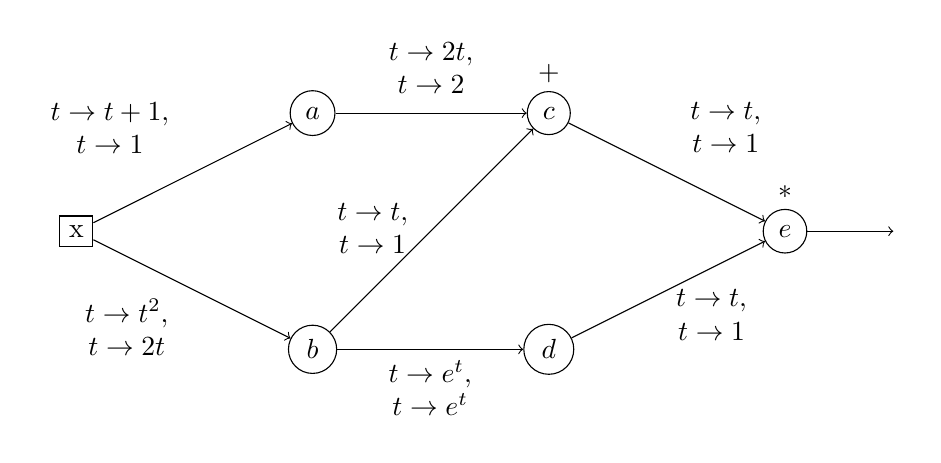
\begin{tikzpicture}
	
		\node[rectangle,draw] (x) at (0,0) {x};
		\node[circle,draw] (a) at (3,1.5) {$a$};
		\node[circle,draw] (b) at (3,-1.5) {$b$};
		\node[circle,draw] (c) at (6,1.5) {$c$};
		\node at (6,2) {$+$};
		\node[circle,draw] (d) at (6,-1.5) {$d$};
		\node[circle,draw] (e) at (9,0) {$e$};
		\node at (9,0.5) {$*$};
		\node (out) at (10.5,0) {};
		
		\path[->] (x) edge node[midway,above left] 
			{$\begin{array}{c}
			 t \to t+1, \\
			 t \to 1
			\end{array}$} (a);
		\path[->] (x) edge node[midway,below left]
			{$\begin{array}{c}
			 t \to t^2, \\
			 t \to 2t
			\end{array}$} (b);
		\path[->] (a) edge node[midway,above] 
			{$\begin{array}{c}
			 t \to 2t, \\
			 t \to 2
			\end{array}$} (c);
			
		\path[->] (b) edge node[midway,left] 
			{$\begin{array}{c}
			 t \to t, \\
			 t \to 1
			\end{array}$} (c);
		\path[->] (b) edge node[midway,below] 
			{$\begin{array}{c}
			 t \to e^t, \\
			 t \to e^t
			\end{array}$} (d);
		\path[->] (c) edge node[midway,above right]
			{$\begin{array}{c}
			 t \to t, \\
			 t \to 1
			\end{array}$} (e);
		\path[->] (d) edge node[midway,below right=-0.2cm] 
			{$\begin{array}{c}
			 t \to t, \\
			 t \to 1
			\end{array}$} (e);
		\path[->] (e) edge (out);
		
	\end{tikzpicture}
	
	\caption{Graphe de calcul de la fonction $f$.}
	\end{figure}

		La figure \ref{fig:graphe_calc_annote_simplement} représente le calcul annoté de la fonction $f$.

	\begin{figure}[!h]
	\label{fig:graphe_calc_annote_simplement}
	\centering
	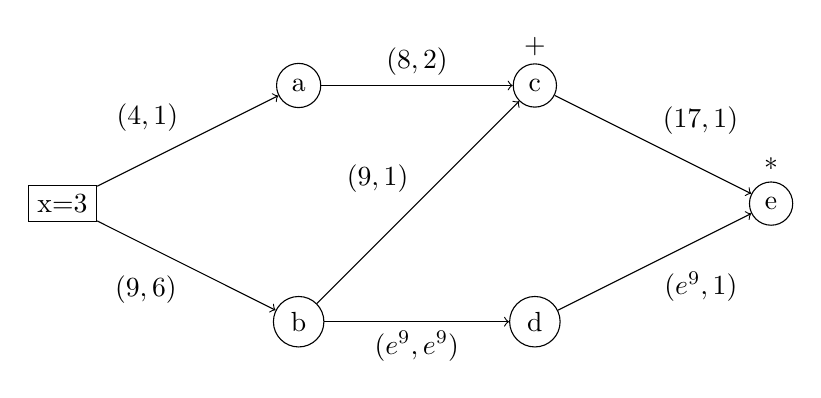
\begin{tikzpicture}
	
		\node[rectangle,draw] (x) at (0,0) {x=3};
		\node[circle,draw] (a) at (3,1.5) {a};
		\node[circle,draw] (b) at (3,-1.5) {b};
		\node[circle,draw] (c) at (6,1.5) {c};
		\node at (6,2) {$+$};
		\node[circle,draw] (d) at (6,-1.5) {d};
		\node[circle,draw] (e) at (9,0) {e};
		\node at (9,0.5) {$*$};
		
		\path[->] (x) edge node[midway,above left] {$(4,1)$} (a);
		\path[->] (x) edge node[midway,below left] {$(9,6)$} (b);
		\path[->] (a) edge node[midway,above] {$(8,2)$} (c);
		\path[->] (b) edge node[midway,above left] {$(9,1)$} (c);
		\path[->] (b) edge node[midway,below] {$(e^9,e^9)$} (d);
		\path[->] (c) edge node[midway,above right] {$(17,1)$} (e);
		\path[->] (d) edge node[midway,below right] {$(e^9,1)$} (e);
		
	\end{tikzpicture}
	
	\caption{Graphe de calcul de la fonction $f$ annoté sur l'exécution $x=3$.}
	\end{figure}


\section{Semi-anneau différentiel}

On introduit ici une notion de semi-anneau différentiel :

\begin{definition}

	Un semi-anneau différentiel $(F,+,\cdot,0,1,d)$ est un semi-anneau commutatif $(F,+,\cdot,0,1)$ muni d'un application $d : F \to F$ vérifiant :
	\begin{itemize}
	
		\item $\forall f,g \in F$, $d(f+g)=d(f)+d(g)$
		
		\item $\forall f,g \in F$, $d(fg)=d(f)g+fd(g)$
			
	\end{itemize}

\end{definition}

L'égalité $d(0 \cdot 0) = d(0)\cdot 0+0\cdot d(0)$ implique $d(0)=0$. En revanche, aucun phénomène analogue ne se produit pour $d(1)$ (c'est le cas dans un anneau différentiel en revanche, car on a l'égalité $d(1) = d(1) + d(1)$).

\section{Executing a computation}

\begin{figure}[!h]
\label{fig:graph_calc_execution}
\centering
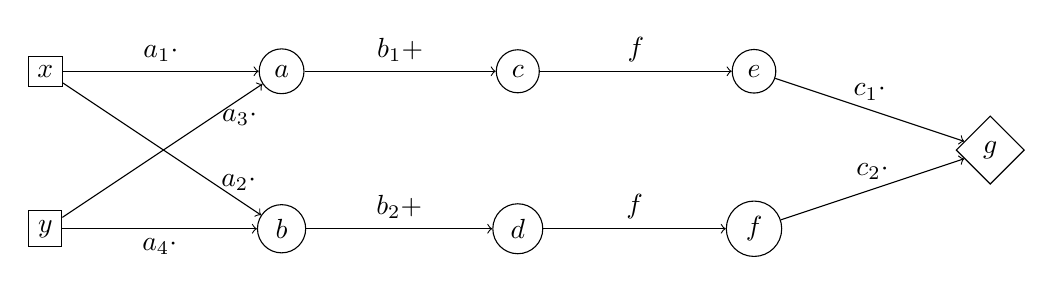
\begin{tikzpicture}

	\def\layersep{3cm}	
	
	\node[rectangle,draw] (x) at (0,1) {$x$};
	\node[rectangle,draw] (y) at (0,-1) {$y$};
	\node[circle,draw] (a) at (\layersep,1) {$a$};
	\node[circle,draw] (b) at (\layersep,-1) {$b$};
	\node[circle,draw] (c) at (2*\layersep,1) {$c$};
	\node[circle,draw] (d) at (2*\layersep,-1) {$d$};
	\node[circle,draw] (e) at (3*\layersep,1) {$e$};
	\node[circle,draw] (f) at (3*\layersep,-1) {$f$};
	\node[diamond,draw] (g) at (4*\layersep,0) {$g$};	
	
	\path[->] (x) edge node[midway,above] {$a_1 \cdot $} (a);
	\path[->] (x) edge node[near end, right] {$a_2 \cdot $} (b);
	\path[->] (y) edge node[near end, right] {$a_3 \cdot$} (a);
	\path[->] (y) edge node[midway,below] {$a_4 \cdot$} (b);
	
	\path[->] (a) edge node[midway,above] {$b_1 + $} (c);
	\path[->] (b) edge node[midway,above] {$b_2 + $} (d);
	
	\path[->] (c) edge node[midway,above] {$f$} (e);
	\path[->] (d) edge node[midway,above] {$f$} (f);
	
	\path[->] (e) edge node[midway,above] {$c_1 \cdot$} (g);
	\path[->] (f) edge node[midway,above] {$c_2 \cdot$} (g);	
	
\end{tikzpicture}
\caption{Executing a computation}
\end{figure}

\ref{fig:graph_calc_execution}

We have a composition and a sum for aggregation. No order for aggregation : + assoc and commut. Composition assoc to treat some modules as black-boxes. Identity and 0 with *1 and *0 (zero-weight is important (no edge)) not sure for *1. $(f+g) \circ h = f \circ h + g \circ h$ ?

\section{Training a model}

Want to add a derivative $d$. Forces to add a $\cdot$. What identities ? -> $d(f \circ g)$ ? 

\section{Cas général}

	\subsection{Définition théorique}

	\begin{definition}
	
	On définit une structure $(F,+,\cdot,\circ,0,1,id,d)$ telle que :
		
		\begin{itemize}
			
			\item $(F,+,\cdot,0,1,d)$ est un semi-anneau différentiel.
			
			\item $(F,\circ,id)$ est un monoïde.
			
			\item Pour tout $(f,g) \in F^2$, $d(f \circ  g) = d(g) \cdot (d(f) \circ g)$.
			
			\item Equalities on $f + g \circ h$ ?
			
		\end{itemize}			
	
	\end{definition}
	
	On modélise un graphe de calcul par un graphe $G=(V,E)$ muni de deux fonctions $fun : E \to F$ et $op : V \to \{+,\cdot\}$.
	
	La fonction $fun$ sert à instancier le calcul.
	
	La fonction $op$ permet de détermier comment aggréger plusieurs fonctions en entrée d'un noeud. Par convention, pour les n\oe uds ayant un degré entrant de $1$, le choix d'opérateur n'a pas d'importance et le n\oe ud est l'identité.\\
	
	Cette définition de la fonction $op$ force l'associativité et la commutativité de $+$ et $\cdot$ (pas d'ordre sur les arrêtes).
	
	\subsection{Exemples}
	
	$\cal{C}^\infty (\R)$,$\cal{C}^\infty (\R^+)$,$\mathbb{R}[X]$,$\mathbb{N}[X]$
	
	\subsection{Objet universel}
	
	\subsection{Remarques}
	
	\begin{enumerate}
	
		\item La factorisation à travers l'objet universel ne peut pas faire apparaitre plus d'informations que l'architecture.
		
		\item Si $op$ est constant égal à $+$, on a la provenance classique.
		
		\item 12
	
	\end{enumerate}
	

\end{document}